\usepackage{mathptmx}
\usepackage{fancyhdr}
\usepackage{appendix}
\usepackage{lipsum}
\usepackage{secdot}
\usepackage{lastpage}
\usepackage{cite}
\usepackage{tabularx}
\usepackage{booktabs}
\usepackage{graphicx}
	\graphicspath{ {images/} }
	
\usepackage{subcaption}
\usepackage{titlesec}
\usepackage{multirow}
\usepackage[hidelinks]{hyperref}

\usepackage{listings}
\usepackage{tocloft}
\usepackage[table,xcdraw]{xcolor}
\usepackage{floatrow}
\floatsetup[table]{capposition=bottom}

\usepackage{ltxtable}

\linespread{1.2}
\pagestyle{fancy}
\fancyhf{} % sets both header and footer to nothing
\renewcommand{\headrulewidth}{0pt}
\rhead{ \textit{FoodFind - A Restaurant Discovery Platform}}
\cfoot{\thepage}

\setlength{\parindent}{0pt}
\setlength{\parskip}{12pt}

\appendix
\begin{document}
\section{APPENDIX}
\subsection{Endpoint: /api/restaurants/}
\usepackage{mathptmx}
\usepackage{fancyhdr}
\usepackage{appendix}
\usepackage{lipsum}
\usepackage{secdot}
\usepackage{lastpage}
\usepackage{cite}
\usepackage{tabularx}
\usepackage{booktabs}
\usepackage{graphicx}
	\graphicspath{ {images/} }
	
\usepackage{subcaption}
\usepackage{titlesec}
\usepackage{multirow}
\usepackage[hidelinks]{hyperref}

\usepackage{listings}
\usepackage{tocloft}
\usepackage[table,xcdraw]{xcolor}
\usepackage{floatrow}
\floatsetup[table]{capposition=bottom}

\usepackage{ltxtable}

\linespread{1.2}
\pagestyle{fancy}
\fancyhf{} % sets both header and footer to nothing
\renewcommand{\headrulewidth}{0pt}
\rhead{ \textit{FoodFind - A Restaurant Discovery Platform}}
\cfoot{\thepage}

\setlength{\parindent}{0pt}
\setlength{\parskip}{12pt}

\appendix
\begin{document}
\section{APPENDIX}
\subsection{Endpoint: /api/restaurants/}
\usepackage{mathptmx}
\usepackage{fancyhdr}
\usepackage{appendix}
\usepackage{lipsum}
\usepackage{secdot}
\usepackage{lastpage}
\usepackage{cite}
\usepackage{tabularx}
\usepackage{booktabs}
\usepackage{graphicx}
	\graphicspath{ {images/} }
	
\usepackage{subcaption}
\usepackage{titlesec}
\usepackage{multirow}
\usepackage[hidelinks]{hyperref}

\usepackage{listings}
\usepackage{tocloft}
\usepackage[table,xcdraw]{xcolor}
\usepackage{floatrow}
\floatsetup[table]{capposition=bottom}

\usepackage{ltxtable}

\linespread{1.2}
\pagestyle{fancy}
\fancyhf{} % sets both header and footer to nothing
\renewcommand{\headrulewidth}{0pt}
\rhead{ \textit{FoodFind - A Restaurant Discovery Platform}}
\cfoot{\thepage}

\setlength{\parindent}{0pt}
\setlength{\parskip}{12pt}

\appendix
\begin{document}
\section{APPENDIX}
\subsection{Endpoint: /api/restaurants/}
\usepackage{mathptmx}
\usepackage{fancyhdr}
\usepackage{appendix}
\usepackage{lipsum}
\usepackage{secdot}
\usepackage{lastpage}
\usepackage{cite}
\usepackage{tabularx}
\usepackage{booktabs}
\usepackage{graphicx}
	\graphicspath{ {images/} }
	
\usepackage{subcaption}
\usepackage{titlesec}
\usepackage{multirow}
\usepackage[hidelinks]{hyperref}

\usepackage{listings}
\usepackage{tocloft}
\usepackage[table,xcdraw]{xcolor}
\usepackage{floatrow}
\floatsetup[table]{capposition=bottom}

\usepackage{ltxtable}

\linespread{1.2}
\pagestyle{fancy}
\fancyhf{} % sets both header and footer to nothing
\renewcommand{\headrulewidth}{0pt}
\rhead{ \textit{FoodFind - A Restaurant Discovery Platform}}
\cfoot{\thepage}

\setlength{\parindent}{0pt}
\setlength{\parskip}{12pt}

\appendix
\begin{document}
\section{APPENDIX}
\subsection{Endpoint: /api/restaurants/}
\input{appendix}
\begin{itemize}
    \item \textbf{Method:} GET
    \item \textbf{Description:} Retrieve a list of restaurants.
    \item \textbf{Parameters:}
    \begin{itemize}
        \item \texttt{tags} (optional): List of tags to filter restaurants by.
    \end{itemize}
    \item \textbf{Response:}
    \begin{verbatim}
    200 OK
    [
        {
            "id": 1,
            "name": "Restaurant Name",
            "location": "Location",
            "description": "Description",
            "images": [
                {
                    "id": 1,
                    "image": "url_to_image"
                }
            ]
        }
    ]
    \end{verbatim}
    \item \textbf{Method:} POST
    \item \textbf{Description:} Create a new restaurant.
    \item \textbf{Request Body:}
    \begin{verbatim}
    {
        "name": "New Restaurant",
        "location": "New Location",
        "description": "New Description",
        "images": [
            {
                "image": "url_to_image"
            }
        ]
    }
    \end{verbatim}
    \item \textbf{Response:}
    \begin{verbatim}
    201 Created
    {
        "id": 2,
        "name": "New Restaurant",
        "location": "New Location",
        "description": "New Description",
        "images": [
            {
                "id": 2,
                "image": "url_to_image"
            }
        ]
    }
    \end{verbatim}
\end{itemize}

\subsection{Endpoint: /api/restaurants/\{id\}/}
\begin{itemize}
    \item \textbf{Method:} GET
    \item \textbf{Description:} Retrieve detailed information about a specific restaurant.
    \item \textbf{Response:}
    \begin{verbatim}
    200 OK
    {
        "id": 1,
        "name": "Restaurant Name",
        "location": "Location",
        "price": "Price",
        "opening_hours": "Opening Hours",
        "description": "Description",
        "average_rating": 4.5,
        "reviews": [
            {
                "id": 1,
                "user": {
                    "id": 1,
                    "username": "User1",
                    "email": "user1@example.com",
                    "profile_picture": "url_to_picture"
                },
                "rating": 5,
                "review_text": "Great place!",
                "created_at": "2024-06-12T00:00:00Z",
                "updated_at": "2024-06-12T00:00:00Z"
            }
        ],
        "map_url": "url_to_map",
        "menu_items": [
            {
                "id": 1,
                "name": "Menu Item",
                "price": "10.99"
            }
        ],
        "no_of_reviews": 10,
        "tags": [
            {
                "id": 1,
                "name": "Tag1"
            }
        ],
        "images": [
            {
                "id": 1,
                "image": "url_to_image"
            }
        ]
    }
    \end{verbatim}
    \item \textbf{Method:} PUT/PATCH
    \item \textbf{Description:} Update a specific restaurant.
    \item \textbf{Request Body:}
    \begin{verbatim}
    {
        "name": "Updated Restaurant Name",
        "location": "Updated Location",
        "description": "Updated Description"
    }
    \end{verbatim}
    \item \textbf{Response:}
    \begin{verbatim}
    200 OK
    {
        "id": 1,
        "name": "Updated Restaurant Name",
        "location": "Updated Location",
        "description": "Updated Description",
        "images": [
            {
                "id": 1,
                "image": "url_to_image"
            }
        ]
    }
    \end{verbatim}
    \item \textbf{Method:} DELETE
    \item \textbf{Description:} Delete a specific restaurant.
    \item \textbf{Response:}
    \begin{verbatim}
    204 No Content
    \end{verbatim}
\end{itemize}

\subsection{Top Restaurant API}

\subsubsection{Endpoint: /api/top-restaurants/}
\begin{itemize}
    \item \textbf{Method:} GET
    \item \textbf{Description:} Retrieve a list of top restaurants.
    \item \textbf{Response:}
    \begin{verbatim}
    200 OK
    [
        {
            "id": 1,
            "restaurant": {
                "id": 1,
                "name": "Top Restaurant",
                "location": "Location",
                "description": "Description",
                "images": [
                    {
                        "id": 1,
                        "image": "url_to_image"
                    }
                ]
            },
            "ranking": 1
        }
    ]
    \end{verbatim}
    \item \textbf{Method:} POST
    \item \textbf{Description:} Create a new top restaurant entry.
    \item \textbf{Request Body:}
    \begin{verbatim}
    {
        "restaurant": 1,
        "ranking": 1
    }
    \end{verbatim}
    \item \textbf{Response:}
    \begin{verbatim}
    201 Created
    {
        "id": 2,
        "restaurant": {
            "id": 1,
            "name": "Top Restaurant",
            "location": "Location",
            "description": "Description",
            "images": [
                {
                    "id": 1,
                    "image": "url_to_image"
                }
            ]
        },
        "ranking": 1
    }
    \end{verbatim}
\end{itemize}


\subsection{Tag API}

\subsubsection{Endpoint: /api/tags/}
\begin{itemize}
    \item \textbf{Method:} GET
    \item \textbf{Description:} Retrieve a list of tags.
    \item \textbf{Response:}
    \begin{verbatim}
    200 OK
    [
        {
            "id": 1,
            "name": "Tag1"
        }
    ]
    \end{verbatim}
    \item \textbf{Method:} POST
    \item \textbf{Description:} Create a new tag.
    \item \textbf{Request Body:}
    \begin{verbatim}
    {
        "name": "New Tag"
    }
    \end{verbatim}
    \item \textbf{Response:}
    \begin{verbatim}
    201 Created
    {
        "id": 2,
        "name": "New Tag"
    }
    \end{verbatim}
\end{itemize}


\subsection{Google Login API}

\subsubsection{Endpoint: /api/auth/google/}
\begin{itemize}
    \item \textbf{Method:} POST
    \item \textbf{Description:} Authenticate a user via Google OAuth.
    \item \textbf{Request Body:}
    \begin{verbatim}
    {
        "token": "google_oauth_token"
    }
    \end{verbatim}
    \item \textbf{Response:}
    \begin{verbatim}
    200 OK
    {
        "id": 1,
        "username": "Username",
        "email": "user@example.com",
        "profile_picture": "http://example.com/user.jpg"
    }
    \end{verbatim}
    \item \textbf{Response on Error:}
    \begin{verbatim}
    400 Bad Request
    {
        "error": "Invalid token"
    }
    \end{verbatim}
\end{itemize}


\subsection{Create Review API}

\subsubsection{Endpoint: /api/reviews/}
\begin{itemize}
    \item \textbf{Method:} POST
    \item \textbf{Description:} Create or update a review for a restaurant.
    \item \textbf{Request Body:}
    \begin{verbatim}
    {
        "user": 1,
        "rating": 5,
        "review_text": "Excellent food!",
        "restaurant": 1
    }
    \end{verbatim}
    \item \textbf{Response:}
    \begin{verbatim}
    200 OK
    {
        "id": 1,
        "user": {
            "id": 1,
            "username": "User1",
            "email": "user1@example.com",
            "profile_picture": "url_to_picture"
        },
        "rating": 5,
        "review_text": "Excellent food!",
        "created_at": "2024-06-12T00:00:00Z",
        "updated_at": "2024-06-12T00:00:00Z"
    }
    \end{verbatim}
    \item \textbf{Response on Error:}
    \begin{verbatim}
    400 Bad Request
    {
        "error": "Validation failed"
    }
    \end{verbatim}
\end{itemize}
\pagebreak

\subsection{OUTPUTS}

\begin{figure}[h]
	\includegraphics[width=\linewidth]{landingpage}
	\centering
	\caption{Home Page}
	\label{fig:Home Page}
\end{figure}

\vspace{7mm}
\begin{figure}[h]
	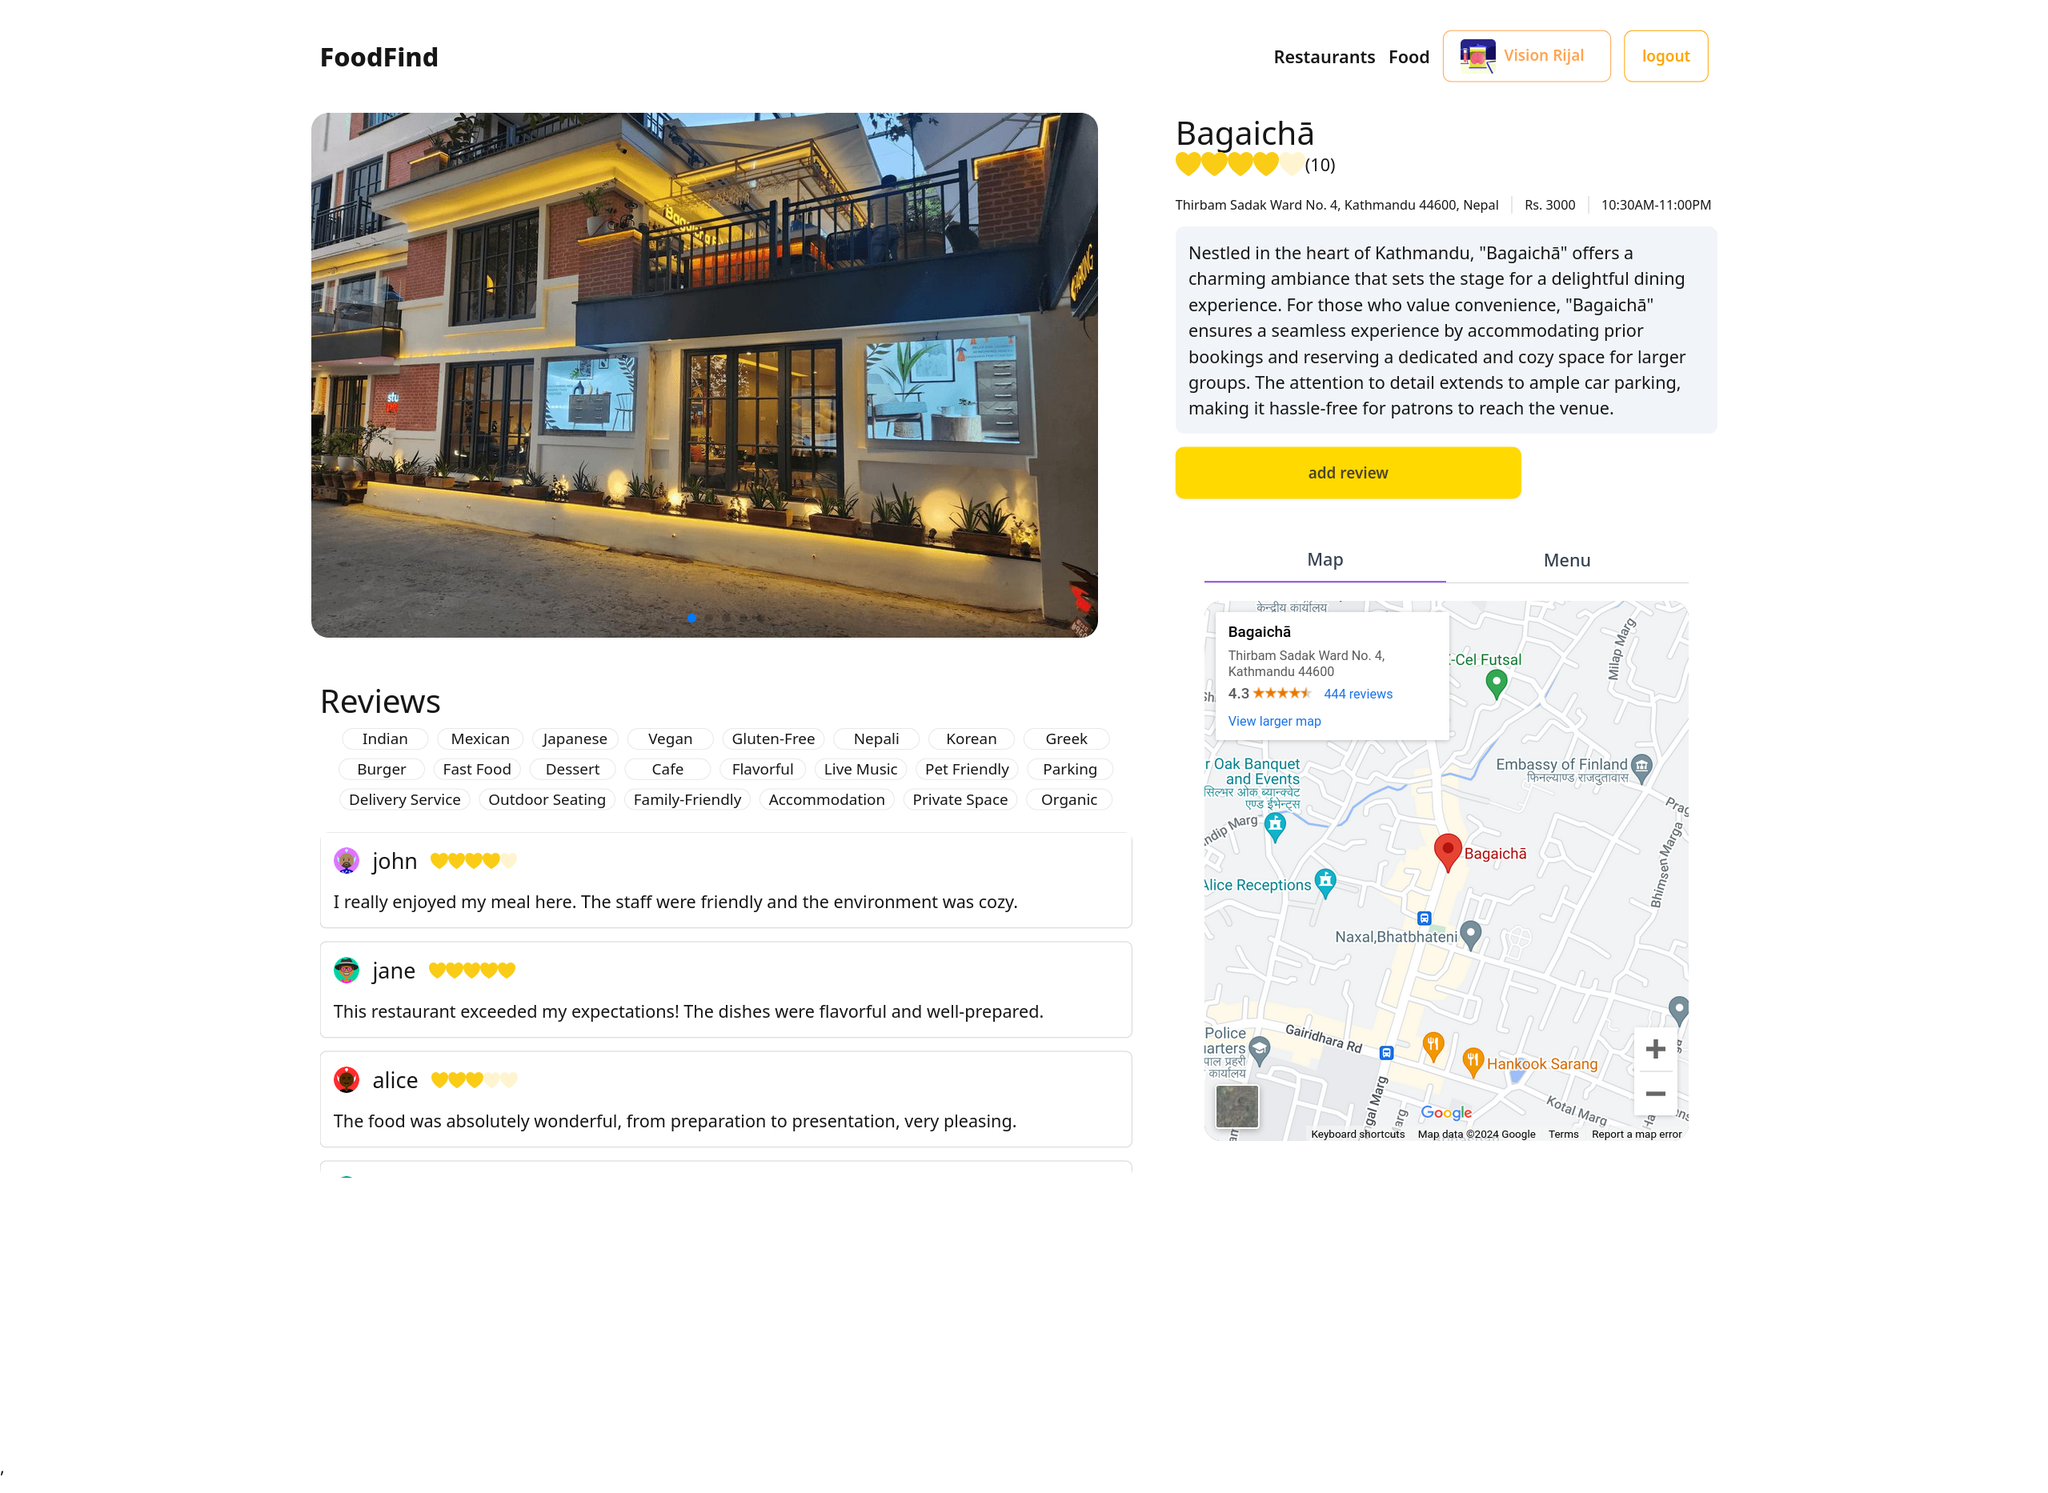
\includegraphics[width=0.8\textwidth]{reviewsdiag}
	\centering
	\caption{Providing Review}
	\label{fig:Review}
\end{figure}


\begin{figure}[h]
	\includegraphics[width=0.9\textwidth]{restaurants}
	\centering
	\caption{Restaurants List}
	\label{fig:Restaurant}
\end{figure}
\end{document}
\begin{itemize}
    \item \textbf{Method:} GET
    \item \textbf{Description:} Retrieve a list of restaurants.
    \item \textbf{Parameters:}
    \begin{itemize}
        \item \texttt{tags} (optional): List of tags to filter restaurants by.
    \end{itemize}
    \item \textbf{Response:}
    \begin{verbatim}
    200 OK
    [
        {
            "id": 1,
            "name": "Restaurant Name",
            "location": "Location",
            "description": "Description",
            "images": [
                {
                    "id": 1,
                    "image": "url_to_image"
                }
            ]
        }
    ]
    \end{verbatim}
    \item \textbf{Method:} POST
    \item \textbf{Description:} Create a new restaurant.
    \item \textbf{Request Body:}
    \begin{verbatim}
    {
        "name": "New Restaurant",
        "location": "New Location",
        "description": "New Description",
        "images": [
            {
                "image": "url_to_image"
            }
        ]
    }
    \end{verbatim}
    \item \textbf{Response:}
    \begin{verbatim}
    201 Created
    {
        "id": 2,
        "name": "New Restaurant",
        "location": "New Location",
        "description": "New Description",
        "images": [
            {
                "id": 2,
                "image": "url_to_image"
            }
        ]
    }
    \end{verbatim}
\end{itemize}

\subsection{Endpoint: /api/restaurants/\{id\}/}
\begin{itemize}
    \item \textbf{Method:} GET
    \item \textbf{Description:} Retrieve detailed information about a specific restaurant.
    \item \textbf{Response:}
    \begin{verbatim}
    200 OK
    {
        "id": 1,
        "name": "Restaurant Name",
        "location": "Location",
        "price": "Price",
        "opening_hours": "Opening Hours",
        "description": "Description",
        "average_rating": 4.5,
        "reviews": [
            {
                "id": 1,
                "user": {
                    "id": 1,
                    "username": "User1",
                    "email": "user1@example.com",
                    "profile_picture": "url_to_picture"
                },
                "rating": 5,
                "review_text": "Great place!",
                "created_at": "2024-06-12T00:00:00Z",
                "updated_at": "2024-06-12T00:00:00Z"
            }
        ],
        "map_url": "url_to_map",
        "menu_items": [
            {
                "id": 1,
                "name": "Menu Item",
                "price": "10.99"
            }
        ],
        "no_of_reviews": 10,
        "tags": [
            {
                "id": 1,
                "name": "Tag1"
            }
        ],
        "images": [
            {
                "id": 1,
                "image": "url_to_image"
            }
        ]
    }
    \end{verbatim}
    \item \textbf{Method:} PUT/PATCH
    \item \textbf{Description:} Update a specific restaurant.
    \item \textbf{Request Body:}
    \begin{verbatim}
    {
        "name": "Updated Restaurant Name",
        "location": "Updated Location",
        "description": "Updated Description"
    }
    \end{verbatim}
    \item \textbf{Response:}
    \begin{verbatim}
    200 OK
    {
        "id": 1,
        "name": "Updated Restaurant Name",
        "location": "Updated Location",
        "description": "Updated Description",
        "images": [
            {
                "id": 1,
                "image": "url_to_image"
            }
        ]
    }
    \end{verbatim}
    \item \textbf{Method:} DELETE
    \item \textbf{Description:} Delete a specific restaurant.
    \item \textbf{Response:}
    \begin{verbatim}
    204 No Content
    \end{verbatim}
\end{itemize}

\subsection{Top Restaurant API}

\subsubsection{Endpoint: /api/top-restaurants/}
\begin{itemize}
    \item \textbf{Method:} GET
    \item \textbf{Description:} Retrieve a list of top restaurants.
    \item \textbf{Response:}
    \begin{verbatim}
    200 OK
    [
        {
            "id": 1,
            "restaurant": {
                "id": 1,
                "name": "Top Restaurant",
                "location": "Location",
                "description": "Description",
                "images": [
                    {
                        "id": 1,
                        "image": "url_to_image"
                    }
                ]
            },
            "ranking": 1
        }
    ]
    \end{verbatim}
    \item \textbf{Method:} POST
    \item \textbf{Description:} Create a new top restaurant entry.
    \item \textbf{Request Body:}
    \begin{verbatim}
    {
        "restaurant": 1,
        "ranking": 1
    }
    \end{verbatim}
    \item \textbf{Response:}
    \begin{verbatim}
    201 Created
    {
        "id": 2,
        "restaurant": {
            "id": 1,
            "name": "Top Restaurant",
            "location": "Location",
            "description": "Description",
            "images": [
                {
                    "id": 1,
                    "image": "url_to_image"
                }
            ]
        },
        "ranking": 1
    }
    \end{verbatim}
\end{itemize}


\subsection{Tag API}

\subsubsection{Endpoint: /api/tags/}
\begin{itemize}
    \item \textbf{Method:} GET
    \item \textbf{Description:} Retrieve a list of tags.
    \item \textbf{Response:}
    \begin{verbatim}
    200 OK
    [
        {
            "id": 1,
            "name": "Tag1"
        }
    ]
    \end{verbatim}
    \item \textbf{Method:} POST
    \item \textbf{Description:} Create a new tag.
    \item \textbf{Request Body:}
    \begin{verbatim}
    {
        "name": "New Tag"
    }
    \end{verbatim}
    \item \textbf{Response:}
    \begin{verbatim}
    201 Created
    {
        "id": 2,
        "name": "New Tag"
    }
    \end{verbatim}
\end{itemize}


\subsection{Google Login API}

\subsubsection{Endpoint: /api/auth/google/}
\begin{itemize}
    \item \textbf{Method:} POST
    \item \textbf{Description:} Authenticate a user via Google OAuth.
    \item \textbf{Request Body:}
    \begin{verbatim}
    {
        "token": "google_oauth_token"
    }
    \end{verbatim}
    \item \textbf{Response:}
    \begin{verbatim}
    200 OK
    {
        "id": 1,
        "username": "Username",
        "email": "user@example.com",
        "profile_picture": "http://example.com/user.jpg"
    }
    \end{verbatim}
    \item \textbf{Response on Error:}
    \begin{verbatim}
    400 Bad Request
    {
        "error": "Invalid token"
    }
    \end{verbatim}
\end{itemize}


\subsection{Create Review API}

\subsubsection{Endpoint: /api/reviews/}
\begin{itemize}
    \item \textbf{Method:} POST
    \item \textbf{Description:} Create or update a review for a restaurant.
    \item \textbf{Request Body:}
    \begin{verbatim}
    {
        "user": 1,
        "rating": 5,
        "review_text": "Excellent food!",
        "restaurant": 1
    }
    \end{verbatim}
    \item \textbf{Response:}
    \begin{verbatim}
    200 OK
    {
        "id": 1,
        "user": {
            "id": 1,
            "username": "User1",
            "email": "user1@example.com",
            "profile_picture": "url_to_picture"
        },
        "rating": 5,
        "review_text": "Excellent food!",
        "created_at": "2024-06-12T00:00:00Z",
        "updated_at": "2024-06-12T00:00:00Z"
    }
    \end{verbatim}
    \item \textbf{Response on Error:}
    \begin{verbatim}
    400 Bad Request
    {
        "error": "Validation failed"
    }
    \end{verbatim}
\end{itemize}
\pagebreak

\subsection{OUTPUTS}

\begin{figure}[h]
	\includegraphics[width=\linewidth]{landingpage}
	\centering
	\caption{Home Page}
	\label{fig:Home Page}
\end{figure}

\vspace{7mm}
\begin{figure}[h]
	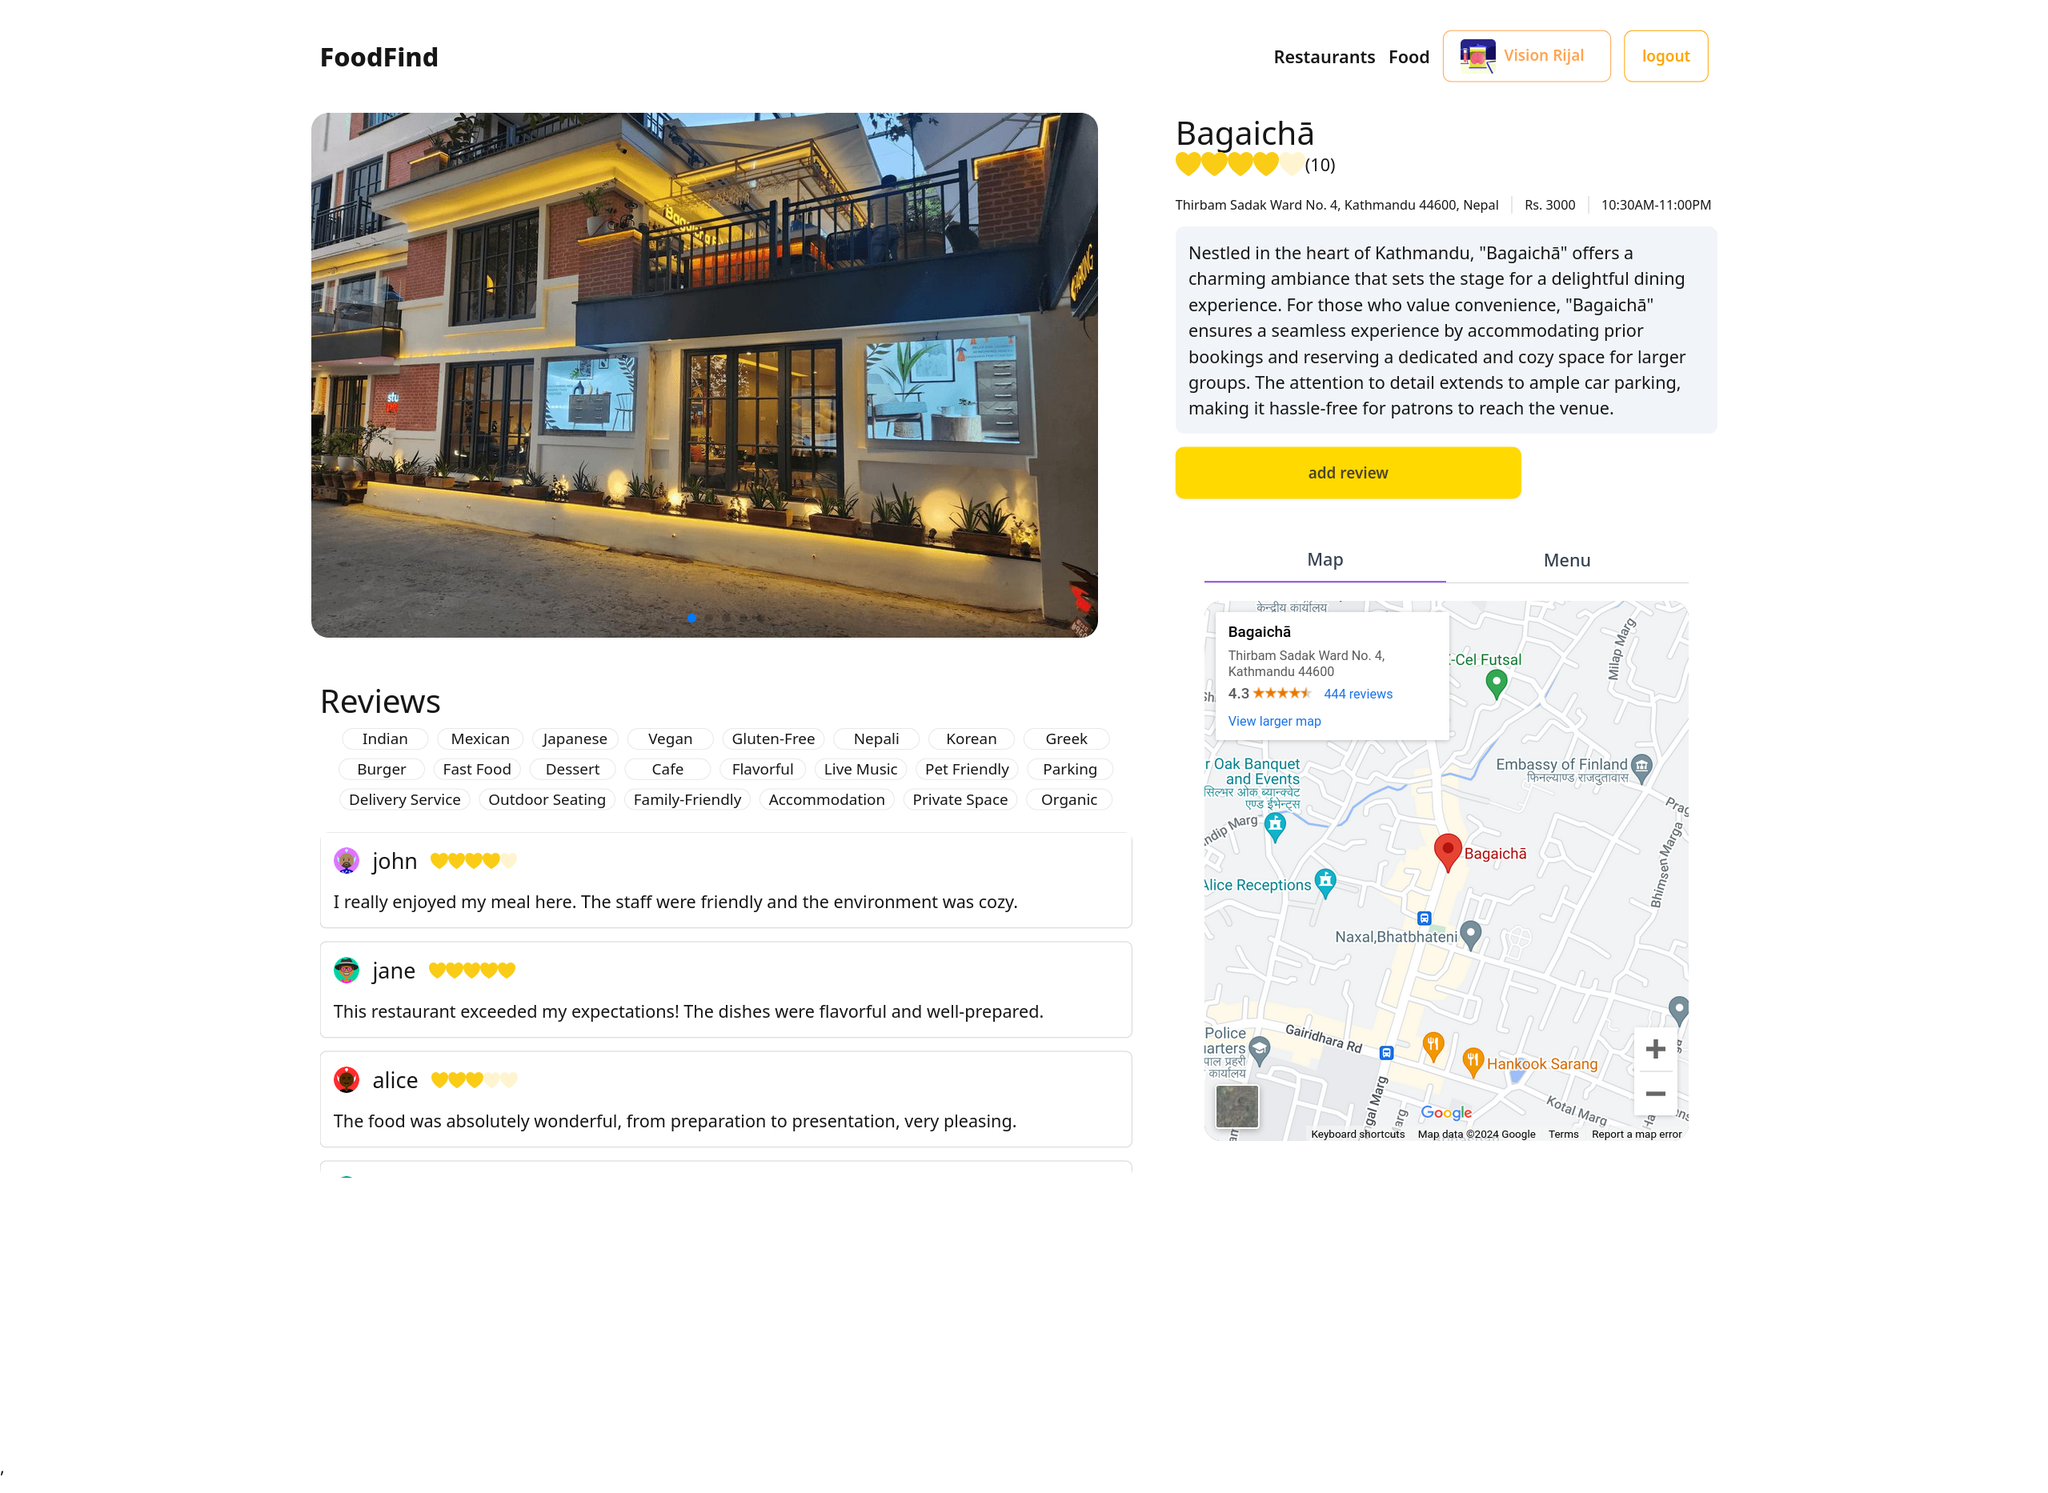
\includegraphics[width=0.8\textwidth]{reviewsdiag}
	\centering
	\caption{Providing Review}
	\label{fig:Review}
\end{figure}


\begin{figure}[h]
	\includegraphics[width=0.9\textwidth]{restaurants}
	\centering
	\caption{Restaurants List}
	\label{fig:Restaurant}
\end{figure}
\end{document}
\begin{itemize}
    \item \textbf{Method:} GET
    \item \textbf{Description:} Retrieve a list of restaurants.
    \item \textbf{Parameters:}
    \begin{itemize}
        \item \texttt{tags} (optional): List of tags to filter restaurants by.
    \end{itemize}
    \item \textbf{Response:}
    \begin{verbatim}
    200 OK
    [
        {
            "id": 1,
            "name": "Restaurant Name",
            "location": "Location",
            "description": "Description",
            "images": [
                {
                    "id": 1,
                    "image": "url_to_image"
                }
            ]
        }
    ]
    \end{verbatim}
    \item \textbf{Method:} POST
    \item \textbf{Description:} Create a new restaurant.
    \item \textbf{Request Body:}
    \begin{verbatim}
    {
        "name": "New Restaurant",
        "location": "New Location",
        "description": "New Description",
        "images": [
            {
                "image": "url_to_image"
            }
        ]
    }
    \end{verbatim}
    \item \textbf{Response:}
    \begin{verbatim}
    201 Created
    {
        "id": 2,
        "name": "New Restaurant",
        "location": "New Location",
        "description": "New Description",
        "images": [
            {
                "id": 2,
                "image": "url_to_image"
            }
        ]
    }
    \end{verbatim}
\end{itemize}

\subsection{Endpoint: /api/restaurants/\{id\}/}
\begin{itemize}
    \item \textbf{Method:} GET
    \item \textbf{Description:} Retrieve detailed information about a specific restaurant.
    \item \textbf{Response:}
    \begin{verbatim}
    200 OK
    {
        "id": 1,
        "name": "Restaurant Name",
        "location": "Location",
        "price": "Price",
        "opening_hours": "Opening Hours",
        "description": "Description",
        "average_rating": 4.5,
        "reviews": [
            {
                "id": 1,
                "user": {
                    "id": 1,
                    "username": "User1",
                    "email": "user1@example.com",
                    "profile_picture": "url_to_picture"
                },
                "rating": 5,
                "review_text": "Great place!",
                "created_at": "2024-06-12T00:00:00Z",
                "updated_at": "2024-06-12T00:00:00Z"
            }
        ],
        "map_url": "url_to_map",
        "menu_items": [
            {
                "id": 1,
                "name": "Menu Item",
                "price": "10.99"
            }
        ],
        "no_of_reviews": 10,
        "tags": [
            {
                "id": 1,
                "name": "Tag1"
            }
        ],
        "images": [
            {
                "id": 1,
                "image": "url_to_image"
            }
        ]
    }
    \end{verbatim}
    \item \textbf{Method:} PUT/PATCH
    \item \textbf{Description:} Update a specific restaurant.
    \item \textbf{Request Body:}
    \begin{verbatim}
    {
        "name": "Updated Restaurant Name",
        "location": "Updated Location",
        "description": "Updated Description"
    }
    \end{verbatim}
    \item \textbf{Response:}
    \begin{verbatim}
    200 OK
    {
        "id": 1,
        "name": "Updated Restaurant Name",
        "location": "Updated Location",
        "description": "Updated Description",
        "images": [
            {
                "id": 1,
                "image": "url_to_image"
            }
        ]
    }
    \end{verbatim}
    \item \textbf{Method:} DELETE
    \item \textbf{Description:} Delete a specific restaurant.
    \item \textbf{Response:}
    \begin{verbatim}
    204 No Content
    \end{verbatim}
\end{itemize}

\subsection{Top Restaurant API}

\subsubsection{Endpoint: /api/top-restaurants/}
\begin{itemize}
    \item \textbf{Method:} GET
    \item \textbf{Description:} Retrieve a list of top restaurants.
    \item \textbf{Response:}
    \begin{verbatim}
    200 OK
    [
        {
            "id": 1,
            "restaurant": {
                "id": 1,
                "name": "Top Restaurant",
                "location": "Location",
                "description": "Description",
                "images": [
                    {
                        "id": 1,
                        "image": "url_to_image"
                    }
                ]
            },
            "ranking": 1
        }
    ]
    \end{verbatim}
    \item \textbf{Method:} POST
    \item \textbf{Description:} Create a new top restaurant entry.
    \item \textbf{Request Body:}
    \begin{verbatim}
    {
        "restaurant": 1,
        "ranking": 1
    }
    \end{verbatim}
    \item \textbf{Response:}
    \begin{verbatim}
    201 Created
    {
        "id": 2,
        "restaurant": {
            "id": 1,
            "name": "Top Restaurant",
            "location": "Location",
            "description": "Description",
            "images": [
                {
                    "id": 1,
                    "image": "url_to_image"
                }
            ]
        },
        "ranking": 1
    }
    \end{verbatim}
\end{itemize}


\subsection{Tag API}

\subsubsection{Endpoint: /api/tags/}
\begin{itemize}
    \item \textbf{Method:} GET
    \item \textbf{Description:} Retrieve a list of tags.
    \item \textbf{Response:}
    \begin{verbatim}
    200 OK
    [
        {
            "id": 1,
            "name": "Tag1"
        }
    ]
    \end{verbatim}
    \item \textbf{Method:} POST
    \item \textbf{Description:} Create a new tag.
    \item \textbf{Request Body:}
    \begin{verbatim}
    {
        "name": "New Tag"
    }
    \end{verbatim}
    \item \textbf{Response:}
    \begin{verbatim}
    201 Created
    {
        "id": 2,
        "name": "New Tag"
    }
    \end{verbatim}
\end{itemize}


\subsection{Google Login API}

\subsubsection{Endpoint: /api/auth/google/}
\begin{itemize}
    \item \textbf{Method:} POST
    \item \textbf{Description:} Authenticate a user via Google OAuth.
    \item \textbf{Request Body:}
    \begin{verbatim}
    {
        "token": "google_oauth_token"
    }
    \end{verbatim}
    \item \textbf{Response:}
    \begin{verbatim}
    200 OK
    {
        "id": 1,
        "username": "Username",
        "email": "user@example.com",
        "profile_picture": "http://example.com/user.jpg"
    }
    \end{verbatim}
    \item \textbf{Response on Error:}
    \begin{verbatim}
    400 Bad Request
    {
        "error": "Invalid token"
    }
    \end{verbatim}
\end{itemize}


\subsection{Create Review API}

\subsubsection{Endpoint: /api/reviews/}
\begin{itemize}
    \item \textbf{Method:} POST
    \item \textbf{Description:} Create or update a review for a restaurant.
    \item \textbf{Request Body:}
    \begin{verbatim}
    {
        "user": 1,
        "rating": 5,
        "review_text": "Excellent food!",
        "restaurant": 1
    }
    \end{verbatim}
    \item \textbf{Response:}
    \begin{verbatim}
    200 OK
    {
        "id": 1,
        "user": {
            "id": 1,
            "username": "User1",
            "email": "user1@example.com",
            "profile_picture": "url_to_picture"
        },
        "rating": 5,
        "review_text": "Excellent food!",
        "created_at": "2024-06-12T00:00:00Z",
        "updated_at": "2024-06-12T00:00:00Z"
    }
    \end{verbatim}
    \item \textbf{Response on Error:}
    \begin{verbatim}
    400 Bad Request
    {
        "error": "Validation failed"
    }
    \end{verbatim}
\end{itemize}
\pagebreak

\subsection{OUTPUTS}

\begin{figure}[h]
	\includegraphics[width=\linewidth]{landingpage}
	\centering
	\caption{Home Page}
	\label{fig:Home Page}
\end{figure}

\vspace{7mm}
\begin{figure}[h]
	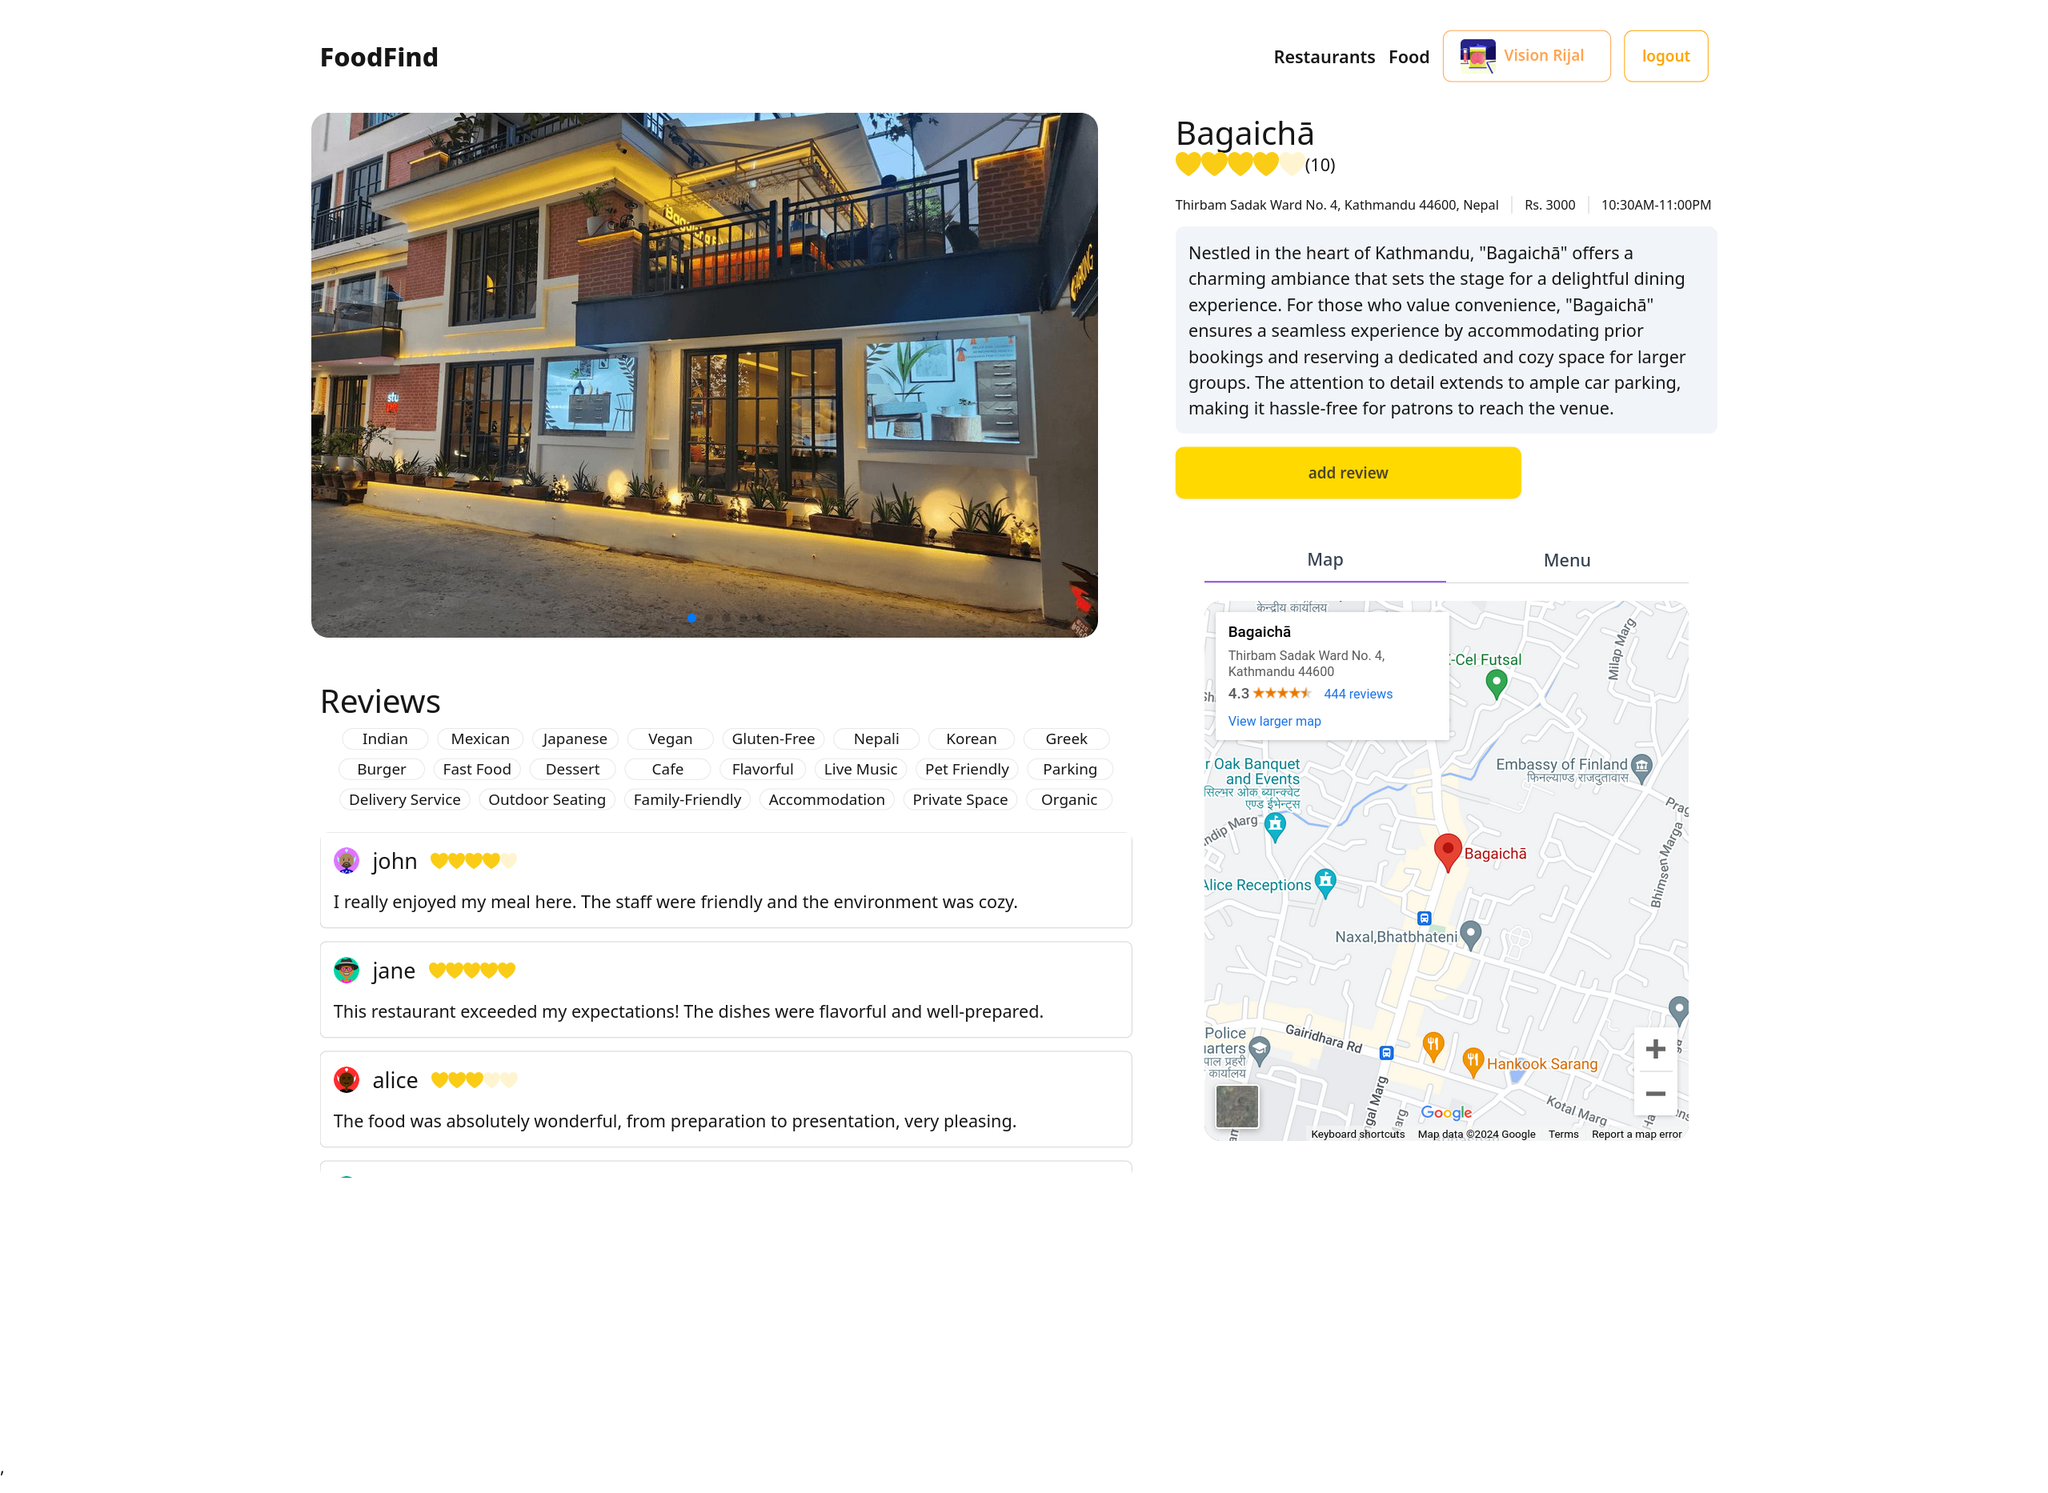
\includegraphics[width=0.8\textwidth]{reviewsdiag}
	\centering
	\caption{Providing Review}
	\label{fig:Review}
\end{figure}


\begin{figure}[h]
	\includegraphics[width=0.9\textwidth]{restaurants}
	\centering
	\caption{Restaurants List}
	\label{fig:Restaurant}
\end{figure}
\end{document}
\begin{itemize}
    \item \textbf{Method:} GET
    \item \textbf{Description:} Retrieve a list of restaurants.
    \item \textbf{Parameters:}
    \begin{itemize}
        \item \texttt{tags} (optional): List of tags to filter restaurants by.
    \end{itemize}
    \item \textbf{Response:}
    \begin{verbatim}
    200 OK
    [
        {
            "id": 1,
            "name": "Restaurant Name",
            "location": "Location",
            "description": "Description",
            "images": [
                {
                    "id": 1,
                    "image": "url_to_image"
                }
            ]
        }
    ]
    \end{verbatim}
    \item \textbf{Method:} POST
    \item \textbf{Description:} Create a new restaurant.
    \item \textbf{Request Body:}
    \begin{verbatim}
    {
        "name": "New Restaurant",
        "location": "New Location",
        "description": "New Description",
        "images": [
            {
                "image": "url_to_image"
            }
        ]
    }
    \end{verbatim}
    \item \textbf{Response:}
    \begin{verbatim}
    201 Created
    {
        "id": 2,
        "name": "New Restaurant",
        "location": "New Location",
        "description": "New Description",
        "images": [
            {
                "id": 2,
                "image": "url_to_image"
            }
        ]
    }
    \end{verbatim}
\end{itemize}

\subsection{Endpoint: /api/restaurants/\{id\}/}
\begin{itemize}
    \item \textbf{Method:} GET
    \item \textbf{Description:} Retrieve detailed information about a specific restaurant.
    \item \textbf{Response:}
    \begin{verbatim}
    200 OK
    {
        "id": 1,
        "name": "Restaurant Name",
        "location": "Location",
        "price": "Price",
        "opening_hours": "Opening Hours",
        "description": "Description",
        "average_rating": 4.5,
        "reviews": [
            {
                "id": 1,
                "user": {
                    "id": 1,
                    "username": "User1",
                    "email": "user1@example.com",
                    "profile_picture": "url_to_picture"
                },
                "rating": 5,
                "review_text": "Great place!",
                "created_at": "2024-06-12T00:00:00Z",
                "updated_at": "2024-06-12T00:00:00Z"
            }
        ],
        "map_url": "url_to_map",
        "menu_items": [
            {
                "id": 1,
                "name": "Menu Item",
                "price": "10.99"
            }
        ],
        "no_of_reviews": 10,
        "tags": [
            {
                "id": 1,
                "name": "Tag1"
            }
        ],
        "images": [
            {
                "id": 1,
                "image": "url_to_image"
            }
        ]
    }
    \end{verbatim}
    \item \textbf{Method:} PUT/PATCH
    \item \textbf{Description:} Update a specific restaurant.
    \item \textbf{Request Body:}
    \begin{verbatim}
    {
        "name": "Updated Restaurant Name",
        "location": "Updated Location",
        "description": "Updated Description"
    }
    \end{verbatim}
    \item \textbf{Response:}
    \begin{verbatim}
    200 OK
    {
        "id": 1,
        "name": "Updated Restaurant Name",
        "location": "Updated Location",
        "description": "Updated Description",
        "images": [
            {
                "id": 1,
                "image": "url_to_image"
            }
        ]
    }
    \end{verbatim}
    \item \textbf{Method:} DELETE
    \item \textbf{Description:} Delete a specific restaurant.
    \item \textbf{Response:}
    \begin{verbatim}
    204 No Content
    \end{verbatim}
\end{itemize}

\subsection{Top Restaurant API}

\subsubsection{Endpoint: /api/top-restaurants/}
\begin{itemize}
    \item \textbf{Method:} GET
    \item \textbf{Description:} Retrieve a list of top restaurants.
    \item \textbf{Response:}
    \begin{verbatim}
    200 OK
    [
        {
            "id": 1,
            "restaurant": {
                "id": 1,
                "name": "Top Restaurant",
                "location": "Location",
                "description": "Description",
                "images": [
                    {
                        "id": 1,
                        "image": "url_to_image"
                    }
                ]
            },
            "ranking": 1
        }
    ]
    \end{verbatim}
    \item \textbf{Method:} POST
    \item \textbf{Description:} Create a new top restaurant entry.
    \item \textbf{Request Body:}
    \begin{verbatim}
    {
        "restaurant": 1,
        "ranking": 1
    }
    \end{verbatim}
    \item \textbf{Response:}
    \begin{verbatim}
    201 Created
    {
        "id": 2,
        "restaurant": {
            "id": 1,
            "name": "Top Restaurant",
            "location": "Location",
            "description": "Description",
            "images": [
                {
                    "id": 1,
                    "image": "url_to_image"
                }
            ]
        },
        "ranking": 1
    }
    \end{verbatim}
\end{itemize}


\subsection{Tag API}

\subsubsection{Endpoint: /api/tags/}
\begin{itemize}
    \item \textbf{Method:} GET
    \item \textbf{Description:} Retrieve a list of tags.
    \item \textbf{Response:}
    \begin{verbatim}
    200 OK
    [
        {
            "id": 1,
            "name": "Tag1"
        }
    ]
    \end{verbatim}
    \item \textbf{Method:} POST
    \item \textbf{Description:} Create a new tag.
    \item \textbf{Request Body:}
    \begin{verbatim}
    {
        "name": "New Tag"
    }
    \end{verbatim}
    \item \textbf{Response:}
    \begin{verbatim}
    201 Created
    {
        "id": 2,
        "name": "New Tag"
    }
    \end{verbatim}
\end{itemize}


\subsection{Google Login API}

\subsubsection{Endpoint: /api/auth/google/}
\begin{itemize}
    \item \textbf{Method:} POST
    \item \textbf{Description:} Authenticate a user via Google OAuth.
    \item \textbf{Request Body:}
    \begin{verbatim}
    {
        "token": "google_oauth_token"
    }
    \end{verbatim}
    \item \textbf{Response:}
    \begin{verbatim}
    200 OK
    {
        "id": 1,
        "username": "Username",
        "email": "user@example.com",
        "profile_picture": "http://example.com/user.jpg"
    }
    \end{verbatim}
    \item \textbf{Response on Error:}
    \begin{verbatim}
    400 Bad Request
    {
        "error": "Invalid token"
    }
    \end{verbatim}
\end{itemize}


\subsection{Create Review API}

\subsubsection{Endpoint: /api/reviews/}
\begin{itemize}
    \item \textbf{Method:} POST
    \item \textbf{Description:} Create or update a review for a restaurant.
    \item \textbf{Request Body:}
    \begin{verbatim}
    {
        "user": 1,
        "rating": 5,
        "review_text": "Excellent food!",
        "restaurant": 1
    }
    \end{verbatim}
    \item \textbf{Response:}
    \begin{verbatim}
    200 OK
    {
        "id": 1,
        "user": {
            "id": 1,
            "username": "User1",
            "email": "user1@example.com",
            "profile_picture": "url_to_picture"
        },
        "rating": 5,
        "review_text": "Excellent food!",
        "created_at": "2024-06-12T00:00:00Z",
        "updated_at": "2024-06-12T00:00:00Z"
    }
    \end{verbatim}
    \item \textbf{Response on Error:}
    \begin{verbatim}
    400 Bad Request
    {
        "error": "Validation failed"
    }
    \end{verbatim}
\end{itemize}
\pagebreak

\subsection{OUTPUTS}

\begin{figure}[h]
	\includegraphics[width=\linewidth]{landingpage}
	\centering
	\caption{Home Page}
	\label{fig:Home Page}
\end{figure}

\vspace{7mm}
\begin{figure}[h]
	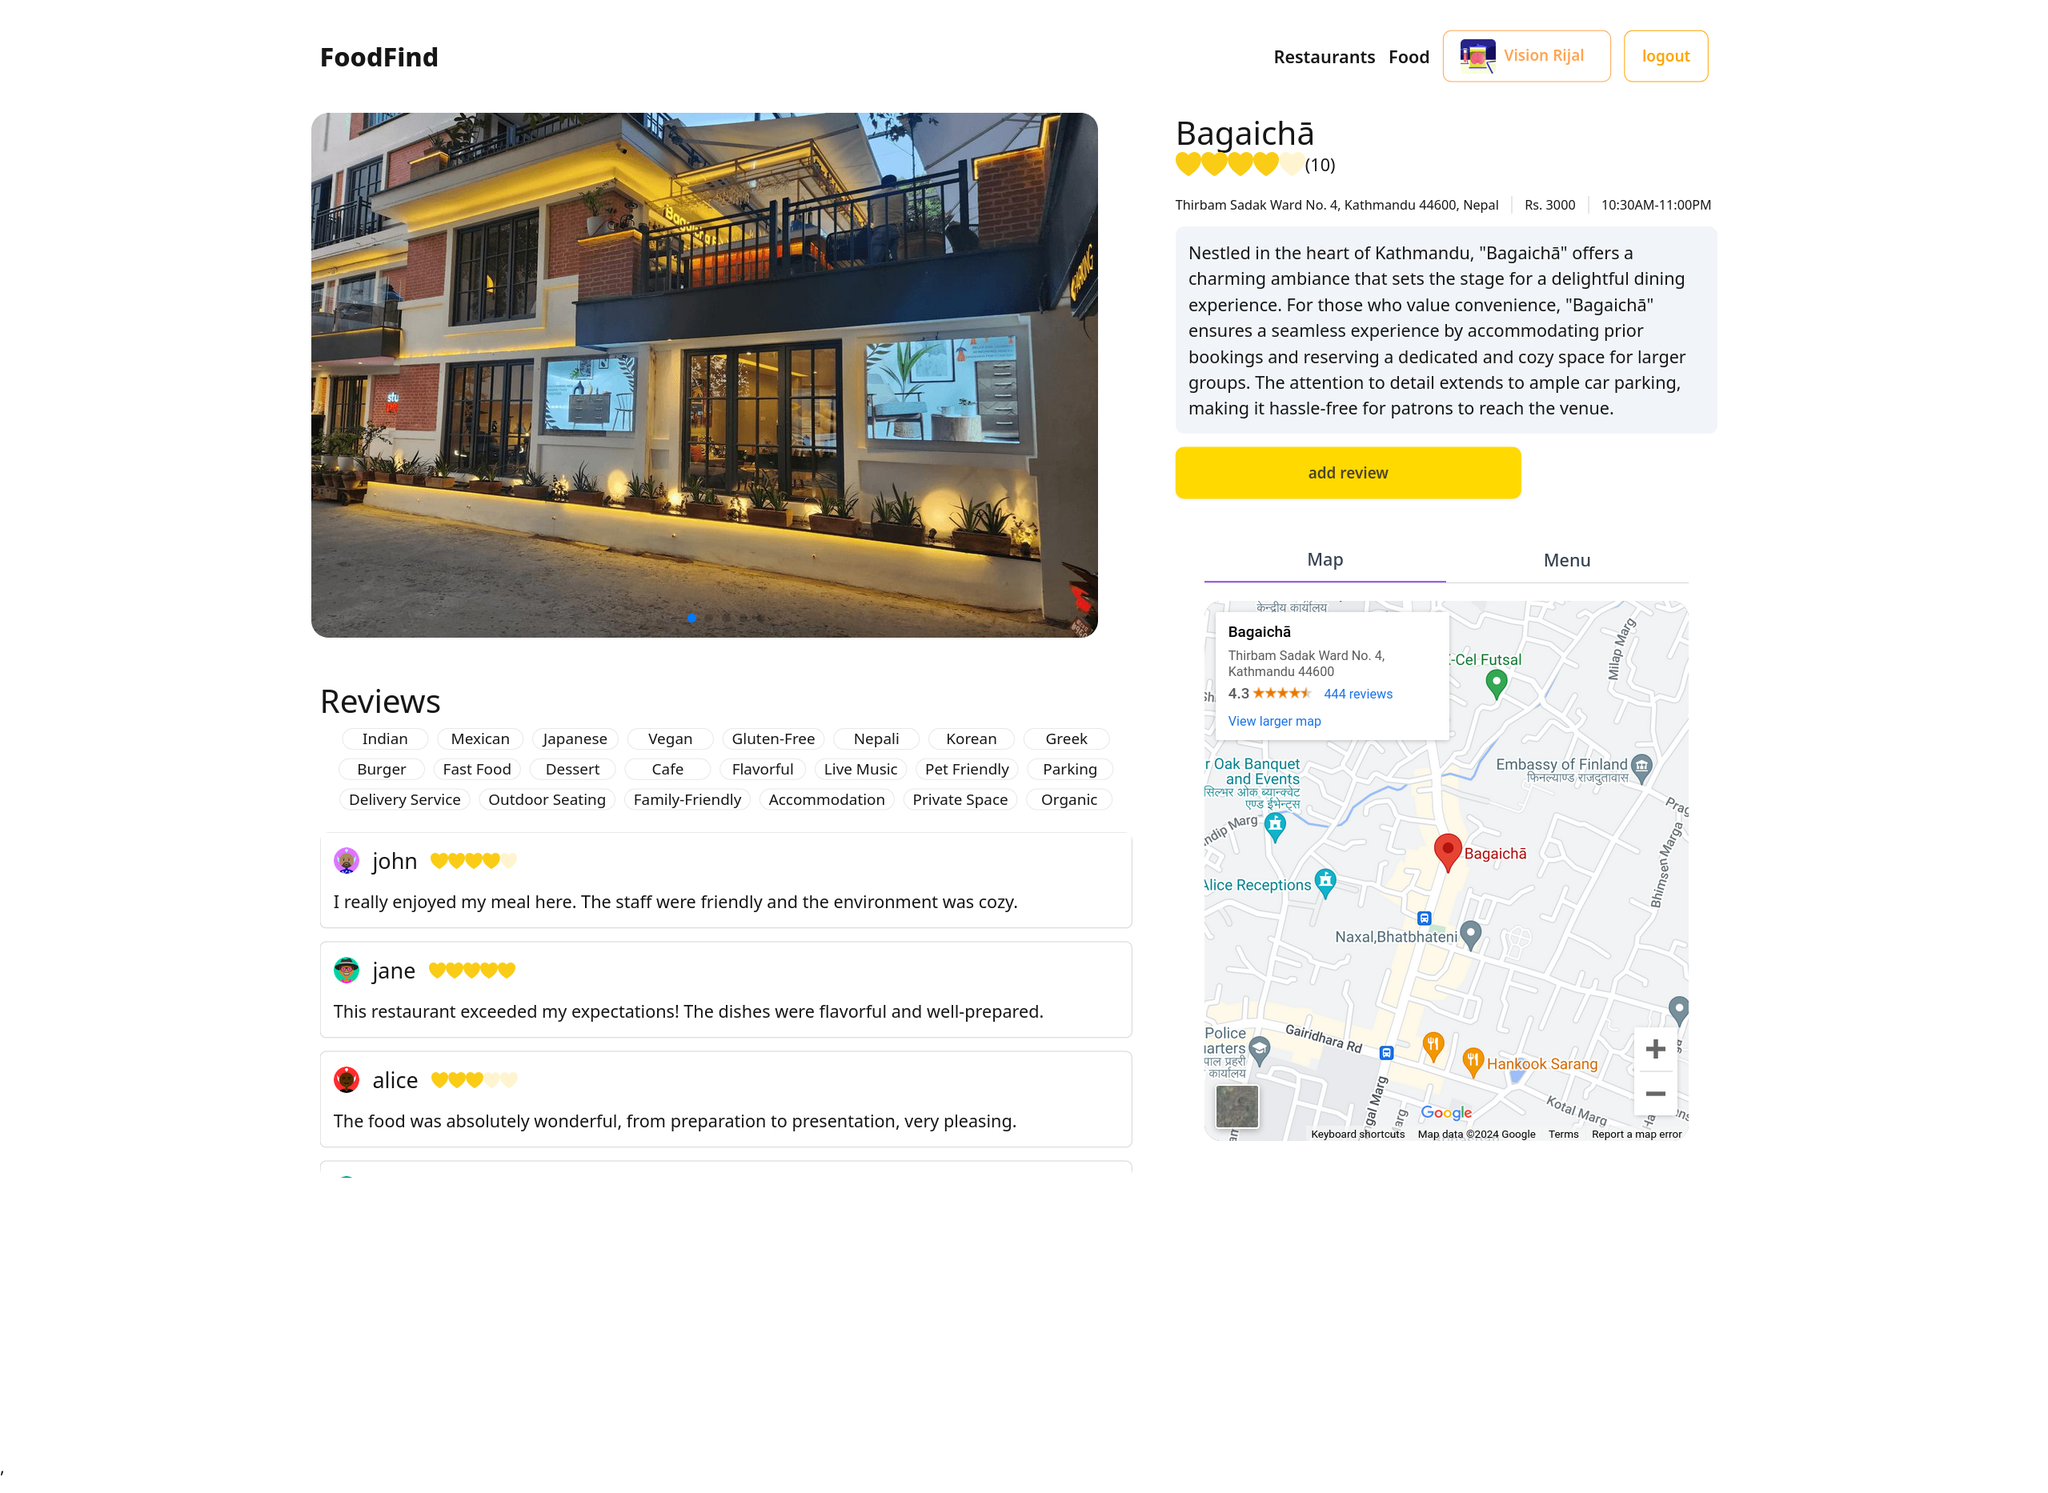
\includegraphics[width=0.8\textwidth]{reviewsdiag}
	\centering
	\caption{Providing Review}
	\label{fig:Review}
\end{figure}


\begin{figure}[h]
	\includegraphics[width=0.9\textwidth]{restaurants}
	\centering
	\caption{Restaurants List}
	\label{fig:Restaurant}
\end{figure}
\end{document}